NB! If the ion relaxes slowly enough, the little extra positive charge "lives" around the lattice point for a long time. Then the electron that caused the lattice fluctuation is long gone. \textbf{Another} electron is then allowed to be pulled towards the positive charge, without the original electron pushing it away, as the repulsive and strong Coulomb interaction is weakened when the distance between the electrons become large.
In other words: by using lattice fluctuations, and by "waiting a little",
\begin{Indentskip}
	\vspace*{-0.5\baselineskip}
	two electrons interact attractively, even if the Coulomb-force (that is repulsive), is taken into account!
\end{Indentskip}
This is quite astonishing, as one naively expects that the Coulomb-forces are \textbf{much} stronger than the weak connection between electrons and phonons.
Remember the Coulomb-potential, we drew it like this:
\begin{feynman}{51}
	\begin{fmfgraph*}(150,65)
		\fmfleftn{i}{2}
		\fmfrightn{o}{2}
		\fmf{fermion}{i1,v1,i2}
		\fmf{fermion}{o1,v2,o2}
		\fmf{photon,label=$\tilde{V}(q)$}{v1,v2}
		\fmfdotn{v}{2}
		\fmflabel{$k,\sigma$}{i1}
		\fmflabel{$k+q,\sigma$}{i2}
		\fmflabel{$k',\sigma'$}{o1}
		\fmflabel{$k'-q,\sigma'$}{o2}
		\fmflabel{$e$}{v1}
		\fmflabel{$e$}{v2}
	\end{fmfgraph*}
\end{feynman}
Coulomb-interaction between the electrons is looked at as an effective interaction between electrons, caused by photons, after an electron-photon-electron interaction. 
The photon-propagator: $\sim\frac{1}{q^2}$.
There is \textbf{no} frequency dependency for \textbf{non}-relativistic electrons: electrons at the Fermi-level have a velocity of $\sim\SI{10e4}{m/s}$. Photons have a velocity of $\sim\SI{3e8}{m/s}$. The interaction between electrons, caused by photons (= Coulomb) is therefore instantaneous: $\delta(t-t')$. The Fourier-transform of a $\delta$ function is a constant. 
For the phonons it is different, the ions relax with velocities much smaller than the electron's, because it has a much greater mass. Therefore the interaction between the electrons caused by phonons is far from instantaneous, it is actually retarded. This means that it takes a long time before the phonon that is emitted from an electron hits another. The diagram, however, stays the same as for the Coulomb-interaction.
\textbf{NB!} We know this from our general considerations around the general form (in a plane-wave basis) of the second quantized form any two-particle operator.
\begin{feynman}{52}
	\begin{fmfgraph*}(150,65)
		\fmfleftn{i}{2}
		\fmfrightn{o}{2}
		\fmf{fermion}{i1,v1,i2}
		\fmf{fermion}{o1,v2,o2}
		\fmf{dashes,label=$D_0(q)$}{v2,v1}
		\fmfdotn{v}{2}
		\fmflabel{$k,\sigma$}{i1}
		\fmflabel{$k+q,\sigma$}{i2}
		\fmflabel{$k',\sigma'$}{o1}
		\fmflabel{$k'-q,\sigma'$}{o2}
		\fmflabel{$M_q$}{v1}
		\fmflabel{$M_q$}{v2}
	\end{fmfgraph*}
\end{feynman}
This is an effective interaction between electrons caused by \textbf{phonons}.
\begin{align}
\label{eq:Veff_electron_phonon}
\tilde{V}_{\text{eff}} = |M_q|^2D_0(q,\omega) = \frac{2|M_q|^2\omega_q}{\omega^2-\omega_q^2}.
\end{align}
When $|\omega|<\omega_q$: $\tilde{V}_{eff} < 0$!
The diagram consists of
\begin{feynman}{53}
\begin{align}
\begin{gathered}
	\begin{fmfgraph*}(65,65)
		\fmfleftn{i}{2}
		\fmfrightn{o}{1}
		\fmf{fermion}{i1,v1,o1}
		\fmf{dashes}{i2,v1}
		\fmfdotn{v}{1}
	\end{fmfgraph*}
	\begin{fmfgraph*}(65,65)
		\fmfleftn{i}{1}
		\fmfrightn{o}{2}
		\fmf{dashes}{v1,o1}
		\fmf{fermion}{i1,v1,o2}
		\fmfdotn{v}{1}
	\end{fmfgraph*}
\end{gathered}
\end{align}
\end{feynman}
$):$ the two vertexes we have in \underline{$V$}. What becomes the effective interaction between \underline{phonons}, caused by electrons, with $V$? The diagram would have to look something like this:
\begin{feynman}{54}
	\begin{fmfgraph*}(150,65)
		\fmfleftn{i}{2}
		\fmfrightn{o}{2}
		\fmf{dashes}{i1,v1,i2}
		\fmf{dashes}{o1,v2,o2}
		\fmf{fermion}{v2,v1}
		\fmfdotn{v}{2}
	\end{fmfgraph*}
\end{feynman}
But something like this does not exist with our $V$, as the vertex
\begin{feynman}{55}
\begin{align}
\begin{gathered}
	\begin{fmfgraph*}(65,65)
		\fmfleftn{i}{2}
		\fmfrightn{o}{1}
		\fmf{dashes}{i1,v1,o1}
		\fmf{fermion}{i2,v1}
		\fmfdotn{v}{1}
	\end{fmfgraph*}
	\begin{fmfgraph*}(65,65)
		\fmfleftn{i}{1}
		\fmfrightn{o}{2}
		\fmf{fermion}{v1,o1}
		\fmf{dashes}{i1,v1,o2}
		\fmfdotn{v}{1}
	\end{fmfgraph*}
\end{gathered}
\end{align}
\end{feynman}
does not exist.
Generally: if we have a potential that couples fermions to a boson, of the type
\begin{align}
\sum_{k, q, \sigma} \lambda_q B_q c_{k+q, \sigma}^{\dagger}c_{k,\sigma}
\end{align}
where the corresponding propagator for the bosons being given by
\begin{align}
D_0(q,t) = -i \hspace{1mm} _0\langle\phi|T\left[B_q(t)B_q(0)^{\dagger}\right]|\phi\rangle_0
\end{align}
then the effective $b_{\omega}$ (?) interaction between the fermions is given by
\begin{align}
V_{eff} = |\lambda_q|^2D_0(q,\omega)+\tilde{V}_{Coulomb}(\vec{q}).
\end{align}
Examples of bosons that have such a link: photons, phonons, magnons (ferromagnetic and antiferromagnetic). (How does a free magnon-propagator look like? Can magnons cause attraction between electrons?)
We look a little closer at $\tilde{V}_{\text{eff}}$ in \eqref{eq:Veff_electron_phonon}. A plot of this potential as a function of $\omega$ is shown in Figure \ref{fig:Veff_electron_phonon}.
\begin{figure}[h!]
\centering
  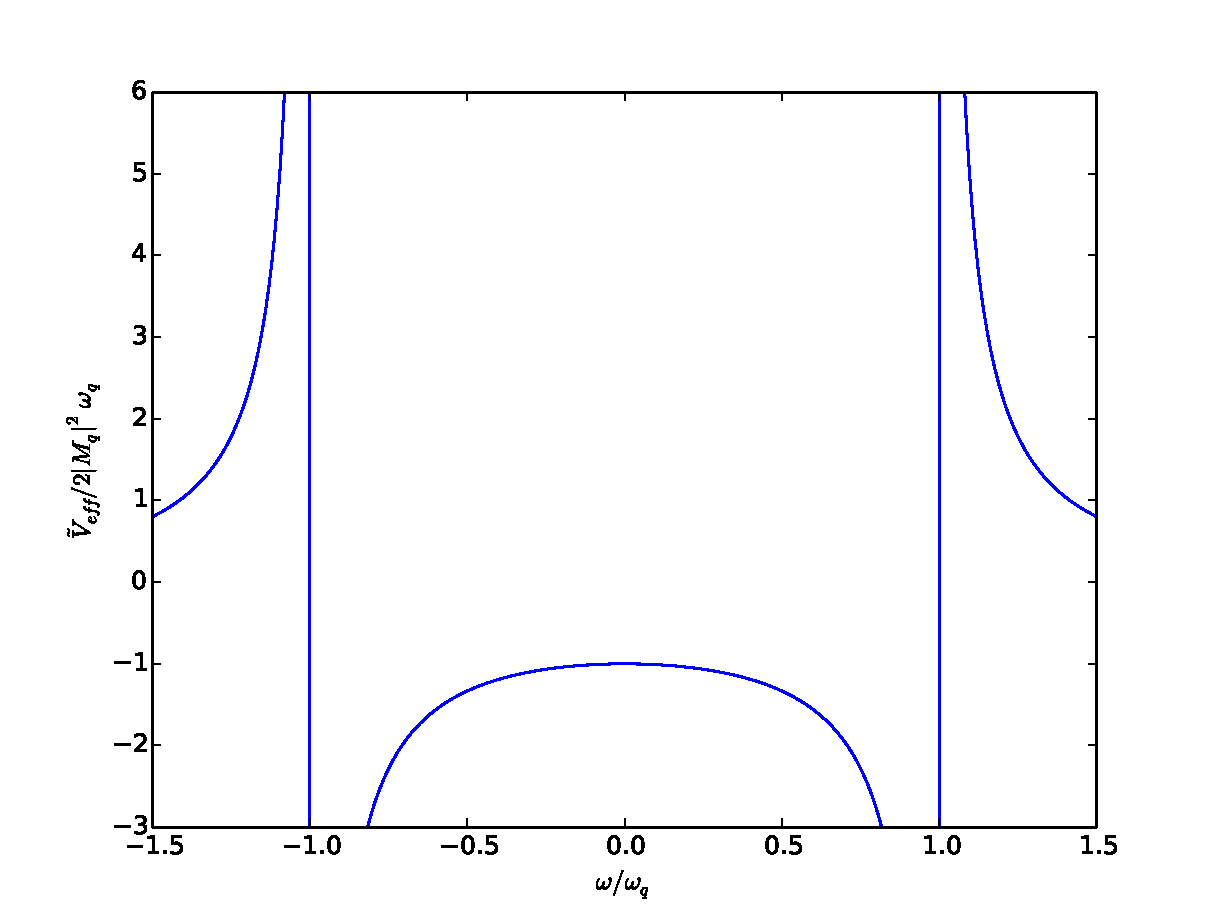
\includegraphics[width=.6\linewidth]{img/veff1.pdf}
  \caption{}
\label{fig:Veff_electron_phonon}
\end{figure}
If we add the Coulomb-interaction, we get a schematical increase $\sim 1/q^2$, which is independent of $\omega$. This is shown in Figure \ref{fig:Veff_electron_phonon_coulomb}. As one can see, there is a small region close to $\pm\omega_q$ where the electrons can only interact attractively. 
\begin{figure}[h!]
\centering
  \includegraphics[width=.6\linewidth]{img/veffCoulomb.pdf}
  \caption{}
\label{fig:Veff_electron_phonon_coulomb}
\end{figure}
Still we \textbf{always} have a small frequency region where the interaction between the electrions become attractive. $\omega$: the energy that is transferred from one electron to another when they collide via phonons (corresponding for other electrons). The electrons that can scatter must be close to the Fermi-level: $\omega\sim\omega_q$ makes $\tilde{V}_{eff}$ large. $\omega_q\sim\omega_D$, the Debye-frequency, which has an order og magnitude $\sim\SI{10e-2}{eV}\sim\SI{100}{K}$. Compared to $\varepsilon_F$, $\omega_q$ is very small. Therefore the involved electrons can only be close to $\varepsilon_F$. The energy transfer $\omega$ is small $\implies$ only electrons in a \textbf{thin shell} $\sim\omega_q\sim\omega_D$ around the Fermi-level can interact attractively via phonons.

\begin{Indentskip}
	\vspace*{-0.5\baselineskip}
	\textbf{NB!} A small frequency corresponds to a long time. The thin shell around the Fermi-level reflects that the second electron must "wait a little" (long time) for the first electron to get away, for the interaction to get attractive.
\end{Indentskip}
\begin{Indentskip}
	\vspace*{-0.5\baselineskip}
	\textbf{NB!} The electrons can not wait too long either, then the lattice has relaxed and there is no positive charge anymore.
\end{Indentskip}

\section{Screening of Coulomb-interaction}
Why does the "free-electron" approximation work well in many metals? That is due to screening, as we will now calculate using Feynman diagrams. Remember Dyson's equation for the \textbf{phonon-propagator:}
\begin{align}
\label{eq:DysonPhononPropagator}
D^{-1} = D_0^{-1} - \Pi \implies D = \frac{D_0}{1 - D_0 \Pi}.
\end{align}
Entirely analogously, we find a Dyson's equation for the photon-propagator, which is the Coulomb-interaction:\\
$D_0(\vec{q}) = \frac{4\pi e^2}{q^2} = V_0$: "Naked" Coulomb-interacton ): Coulomb-interaction between two isolated electrons.\\
$D$: Renormalized photon-propagator ): renormalized Coulomb-potential.\\
\textbf{Diagrammatically}:
\begin{feynman}{56DysonEq}
\begin{align}
D &=
\begin{gathered}
	\begin{fmfgraph*}(40,25)
		\fmfleftn{i}
		\fmfrightn{o}
		\fmf{dbl_wiggly}{i,o}
	\end{fmfgraph*}
\end{gathered} \\
D_0 &=
\begin{gathered}
	\begin{fmfgraph*}(40,25)
		\fmfleftn{i}
		\fmfrightn{o}
		\fmf{wiggly}{i,o}
	\end{fmfgraph*}
\end{gathered} \\
\nonumber D &= \begin{gathered}
	\begin{fmfgraph*}(40,25)
		\fmfleftn{i}
		\fmfrightn{o}
		\fmf{wiggly}{i,o}
	\end{fmfgraph*}
	+
	\begin{fmfgraph*}(40,40)
		\fmfleftn{i}
		\fmfrightn{o}
		\fmf{wiggly,tension=5}{i,v1}
		\fmf{wiggly,tension=5}{v2,o}
		\fmf{plain,left,tension=0.4}{v1,v2,v1}
		\fmfdot{v1,v2}
	\end{fmfgraph*}
\end{gathered} \\
\nonumber &+
\begin{gathered}
	\begin{fmfgraph*}(60,40)
		\fmfleftn{i}
		\fmfrightn{o}
		\fmf{wiggly,tension=5}{i,v1}
		\fmf{wiggly,tension=5}{v2,o}
		\fmf{fermion,left,tension=0.4}{i1,v1,i1}
		\fmf{fermion,left,tension=0.4}{o1,v2,o1}
		\fmf{wiggly}{v1,v2}
	\end{fmfgraph*}
\end{gathered} \\
&+
\begin{gathered}
	\begin{fmfgraph*}(40,40)
		\fmfleftn{i}
		\fmfrightn{o}
		\fmf{wiggly,tension=5}{i,v1}
		\fmf{wiggly,tension=5}{v3,o}
		\fmf{plain,left,tension=0.4}{v1,v2,v3,v4,v1}
		\fmf{wiggly,tension=5}{v2,v4}
	\end{fmfgraph*}
	+
	\begin{fmfgraph*}(40,40)
		\fmfleftn{i}
		\fmfrightn{o}
		\fmf{wiggly,tension=5}{i,v1}
		\fmf{wiggly,tension=5}{v4,o}
		\fmf{plain,left,tension=0.4}{v1,v2,v3,v4,v1}
		\fmf{photon,left=0.5,tension=0.2}{v2,v3}
	\end{fmfgraph*}
\end{gathered} + \ldots
\end{align}
\end{feynman}
We now make the following approximation: instead of doing \textit{pure} perturbation theory, we sum all the diagrams of one particular type to the order of infinity:
\begin{feynman}{57DysonApprox}
\begin{align}
D &\approx
\begin{gathered}
	\begin{fmfgraph*}(40,25)
		\fmfleftn{i}
		\fmfrightn{o}
		\fmf{wiggly}{i,o}
	\end{fmfgraph*}
\end{gathered} \\
\nonumber D &= \begin{gathered}
	\begin{fmfgraph*}(40,25)
		\fmfleftn{i}
		\fmfrightn{o}
		\fmf{wiggly}{i,o}
	\end{fmfgraph*}
	+
	\begin{fmfgraph*}(40,40)
		\fmfleftn{i}
		\fmfrightn{o}
		\fmf{wiggly,tension=5}{i,v1}
		\fmf{wiggly,tension=5}{v2,o}
		\fmf{plain,left,tension=0.4}{v1,v2,v1}
		\fmfdot{v1,v2}
	\end{fmfgraph*}
	+
	\begin{fmfgraph*}(60,40)
		\fmfleftn{i}
		\fmfrightn{o}
		\fmf{wiggly,tension=5}{i,v1}
		\fmf{wiggly,tension=5}{v2,o}
		\fmf{fermion,left,tension=0.4}{i1,v1,i1}
		\fmf{fermion,left,tension=0.4}{o1,v2,o1}
		\fmf{wiggly}{v1,v2}
	\end{fmfgraph*}
\end{gathered} \\
\nonumber &+
\begin{gathered}
	\begin{fmfgraph*}(60,40)
		\fmfleftn{i}
		\fmfrightn{o}
		\fmf{wiggly,tension=5}{i,v1}
		\fmf{wiggly,tension=5}{v2,o}
		\fmf{fermion,left,tension=0.4}{i1,v1,i1}
		\fmf{fermion,left,tension=0.4}{v2,v3,v2}
		\fmf{fermion,left,tension=0.4}{o1,v4,o1}
		\fmf{wiggly}{v1,v2}
		\fmf{wiggly}{v2,v3}
	\end{fmfgraph*}
\end{gathered} + \ldots \\
&=
\begin{fmfgraph*}(40,20)
		\fmfleftn{i}
		\fmfrightn{o}
		\fmf{wiggly}{i,o}
\end{fmfgraph*}
\left[
1 +
\begin{fmfgraph*}(40,20)
		\fmfleftn{i}
		\fmfrightn{o}
		\fmf{wiggly,tension=5}{i,v1}
		\fmf{phantom,tension=5}{v2,o}
		\fmf{plain,left,tension=0.4}{v1,v2,v1}
		\fmfdot{v1,v2}
\end{fmfgraph*}
+
\left(
\begin{fmfgraph*}(40,20)
		\fmfleftn{i}
		\fmfrightn{o}
		\fmf{wiggly,tension=5}{i,v1}
		\fmf{phantom,tension=5}{v2,o}
		\fmf{plain,left,tension=0.4}{v1,v2,v1}
		\fmfdot{v1,v2}
\end{fmfgraph*}
\right)^2
+
\left(
\begin{fmfgraph*}(40,20)
		\fmfleftn{i}
		\fmfrightn{o}
		\fmf{wiggly,tension=5}{i,v1}
		\fmf{phantom,tension=5}{v2,o}
		\fmf{plain,left,tension=0.4}{v1,v2,v1}
		\fmfdot{v1,v2}
\end{fmfgraph*}
\right)^3
+\ldots
\right].
\end{align}
\end{feynman}
The content between the brackets is recognized as a geometric series, the sum of which is known as
\begin{align}
\sum_{n=0}^{\infty} x^n = \frac{1}{1-x}.
\end{align}
This gives us
\begin{feynman}{58DysonGeometricSeries}
\begin{align}
\nonumber D(q,\omega) &= 
\begin{gathered}
\frac{\begin{fmfgraph*}(40,25)
		\fmfleftn{i}
		\fmfrightn{o}
		\fmf{wiggly}{i,o}
\end{fmfgraph*}}{1-\begin{fmfgraph*}(40,20)
		\fmfleftn{i}
		\fmfrightn{o}
		\fmf{wiggly,tension=5}{i,v1}
		\fmf{phantom,tension=5}{v2,o}
		\fmf{plain,left,tension=0.4}{v1,v2,v1}
		\fmfdot{v1,v2}
\end{fmfgraph*}}
\end{gathered}
= \frac{V_0(q)}{1-V_0(q)\Pi^2(q,\omega)} \\
&= \frac{4\pi e^2}{q^2}\frac{1}{\varepsilon(q,\omega)}.
\end{align}
\end{feynman}
Here $\varepsilon(q,\omega) = 1-V_0(q)\Pi^{(2)}(q,\omega)$ is the dielectric constant. This we have to calculate, which means we have to calculate the feynman diagram
\begin{feynman}{59Loop}
\begin{fmfgraph*}(40,20)
		\fmfleftn{i}
		\fmfrightn{o}
		\fmf{phantom,tension=5}{i,v1}
		\fmf{phantom,tension=5}{v2,o}
		\fmf{plain,left,tension=0.4}{v1,v2,v1}
		\fmfdot{v1,v2}
\end{fmfgraph*}
\end{feynman}.
\subsection{Calculation of \texorpdfstring{$\Pi^{(2)}(q,\omega)$}{pi(q,omega)}}
\begin{feynman}{60pi2}
	\begin{fmfgraph*}(150,65)
		\fmfleftn{i}
		\fmfrightn{o}
		\fmf{dashes}{i,v1}
		\fmf{dashes}{v2,o}
		\fmf{fermion,label=$k+q, \omega+\omega '$}{v1,v2}
		\fmf{fermion,label=$k, \omega '$}{v2,v1}
		\fmfdotn{v}{2}
		\fmflabel{$q,\omega$}{i}
		\fmflabel{$q,\omega$}{o}
	\end{fmfgraph*}
\end{feynman}
Use the Feynman rules. $F = 1$: number of vertexes $=2$ $\implies$ $m=1$. The prefactor is
\begin{align}
i(-1)^1(2\cdot\frac{1}{2}+1)^1\sum_{k,q} \int_{-\infty}^{\infty}\frac{\textrm{d} \omega'}{2\pi} G_0(k+q,\omega+\omega')\cdot G(k,\omega').
\end{align}
Remember that
\begin{align}
G_0(k,\omega) = \frac{\theta(\varepsilon_k-\varepsilon_F)}{\omega-\varepsilon_k+i\delta} + \frac{\theta(\varepsilon_F-\varepsilon_k)}{\omega-\varepsilon_k-i\delta}.
\end{align}
We do the frequency integral first by contour-integration and residue calculation. $\int_{-\infty}^{\infty}\textrm{d} x \rightarrow \int_C\textrm{d} z$, with $C$ being a curve in the complex plane that closes the integral over $x$. Whether we close the integral in the upper or lower part of the complex plane is up to us.